\documentclass{standalone}
\usepackage{tikz,xcolor-material}
\begin{document}
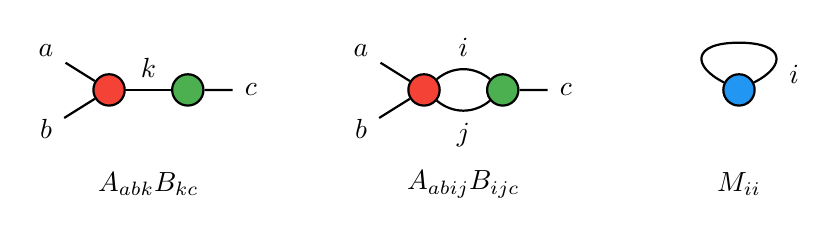
\begin{tikzpicture}[inner sep=4pt, thick]
  \path node (A1)  at (0,0) [circle, draw, fill=MaterialRed] {}
        node (B1)  at (1,0) [circle, draw, fill=MaterialGreen] {}
        node (A1a) at (-0.8, 0.5) {$a$}
        node (A1b) at (-0.8,-0.5) {$b$}
        node (B1c) at (1.8,0)     {$c$}
        %
        node (A2)  at (4,0) [circle, draw, fill=MaterialRed] {}
        node (B2)  at (5,0) [circle, draw, fill=MaterialGreen] {}
        node (A2a) at (3.2, 0.5) {$a$}
        node (A2b) at (3.2,-0.5) {$b$}
        node (B2c) at (5.8,0)    {$c$}
        %
        node (M)   at (8,0) [circle, draw, fill=MaterialBlue] {}
        %
        node at (0.5,-1.2) {$A_{abk} B_{kc}$}
        node at (4.5,-1.2) {$A_{abij} B_{ijc}$}
        node at (  8,-1.2) {$M_{ii}$};
  \draw (A1) edge [above] node {$k$} (B1)
        (A1) -- (A1a)
        (A1) -- (A1b)
        (B1) -- (B1c)
        %
        (A2) to [bend left=40,  above] node {$i$} (B2)
        (A2) to [bend right=40, below] node {$j$} (B2)
        (A2) -- (A2a)
        (A2) -- (A2b)
        (B2) -- (B2c)
        %
        (M) .. controls (7.4,0.3) and (7.4,0.6) .. (8,0.6)
            .. controls (8.6,0.6) and (8.6,0.3) .. (M) node at (8.7,0.2) {$i$};
\end{tikzpicture}
\end{document}
